% Options for packages loaded elsewhere
\PassOptionsToPackage{unicode}{hyperref}
\PassOptionsToPackage{hyphens}{url}
%
\documentclass[
]{book}
\usepackage{amsmath,amssymb}
\usepackage{iftex}
\ifPDFTeX
  \usepackage[T1]{fontenc}
  \usepackage[utf8]{inputenc}
  \usepackage{textcomp} % provide euro and other symbols
\else % if luatex or xetex
  \usepackage{unicode-math} % this also loads fontspec
  \defaultfontfeatures{Scale=MatchLowercase}
  \defaultfontfeatures[\rmfamily]{Ligatures=TeX,Scale=1}
\fi
\usepackage{lmodern}
\ifPDFTeX\else
  % xetex/luatex font selection
\fi
% Use upquote if available, for straight quotes in verbatim environments
\IfFileExists{upquote.sty}{\usepackage{upquote}}{}
\IfFileExists{microtype.sty}{% use microtype if available
  \usepackage[]{microtype}
  \UseMicrotypeSet[protrusion]{basicmath} % disable protrusion for tt fonts
}{}
\makeatletter
\@ifundefined{KOMAClassName}{% if non-KOMA class
  \IfFileExists{parskip.sty}{%
    \usepackage{parskip}
  }{% else
    \setlength{\parindent}{0pt}
    \setlength{\parskip}{6pt plus 2pt minus 1pt}}
}{% if KOMA class
  \KOMAoptions{parskip=half}}
\makeatother
\usepackage{xcolor}
\usepackage{color}
\usepackage{fancyvrb}
\newcommand{\VerbBar}{|}
\newcommand{\VERB}{\Verb[commandchars=\\\{\}]}
\DefineVerbatimEnvironment{Highlighting}{Verbatim}{commandchars=\\\{\}}
% Add ',fontsize=\small' for more characters per line
\usepackage{framed}
\definecolor{shadecolor}{RGB}{248,248,248}
\newenvironment{Shaded}{\begin{snugshade}}{\end{snugshade}}
\newcommand{\AlertTok}[1]{\textcolor[rgb]{0.94,0.16,0.16}{#1}}
\newcommand{\AnnotationTok}[1]{\textcolor[rgb]{0.56,0.35,0.01}{\textbf{\textit{#1}}}}
\newcommand{\AttributeTok}[1]{\textcolor[rgb]{0.13,0.29,0.53}{#1}}
\newcommand{\BaseNTok}[1]{\textcolor[rgb]{0.00,0.00,0.81}{#1}}
\newcommand{\BuiltInTok}[1]{#1}
\newcommand{\CharTok}[1]{\textcolor[rgb]{0.31,0.60,0.02}{#1}}
\newcommand{\CommentTok}[1]{\textcolor[rgb]{0.56,0.35,0.01}{\textit{#1}}}
\newcommand{\CommentVarTok}[1]{\textcolor[rgb]{0.56,0.35,0.01}{\textbf{\textit{#1}}}}
\newcommand{\ConstantTok}[1]{\textcolor[rgb]{0.56,0.35,0.01}{#1}}
\newcommand{\ControlFlowTok}[1]{\textcolor[rgb]{0.13,0.29,0.53}{\textbf{#1}}}
\newcommand{\DataTypeTok}[1]{\textcolor[rgb]{0.13,0.29,0.53}{#1}}
\newcommand{\DecValTok}[1]{\textcolor[rgb]{0.00,0.00,0.81}{#1}}
\newcommand{\DocumentationTok}[1]{\textcolor[rgb]{0.56,0.35,0.01}{\textbf{\textit{#1}}}}
\newcommand{\ErrorTok}[1]{\textcolor[rgb]{0.64,0.00,0.00}{\textbf{#1}}}
\newcommand{\ExtensionTok}[1]{#1}
\newcommand{\FloatTok}[1]{\textcolor[rgb]{0.00,0.00,0.81}{#1}}
\newcommand{\FunctionTok}[1]{\textcolor[rgb]{0.13,0.29,0.53}{\textbf{#1}}}
\newcommand{\ImportTok}[1]{#1}
\newcommand{\InformationTok}[1]{\textcolor[rgb]{0.56,0.35,0.01}{\textbf{\textit{#1}}}}
\newcommand{\KeywordTok}[1]{\textcolor[rgb]{0.13,0.29,0.53}{\textbf{#1}}}
\newcommand{\NormalTok}[1]{#1}
\newcommand{\OperatorTok}[1]{\textcolor[rgb]{0.81,0.36,0.00}{\textbf{#1}}}
\newcommand{\OtherTok}[1]{\textcolor[rgb]{0.56,0.35,0.01}{#1}}
\newcommand{\PreprocessorTok}[1]{\textcolor[rgb]{0.56,0.35,0.01}{\textit{#1}}}
\newcommand{\RegionMarkerTok}[1]{#1}
\newcommand{\SpecialCharTok}[1]{\textcolor[rgb]{0.81,0.36,0.00}{\textbf{#1}}}
\newcommand{\SpecialStringTok}[1]{\textcolor[rgb]{0.31,0.60,0.02}{#1}}
\newcommand{\StringTok}[1]{\textcolor[rgb]{0.31,0.60,0.02}{#1}}
\newcommand{\VariableTok}[1]{\textcolor[rgb]{0.00,0.00,0.00}{#1}}
\newcommand{\VerbatimStringTok}[1]{\textcolor[rgb]{0.31,0.60,0.02}{#1}}
\newcommand{\WarningTok}[1]{\textcolor[rgb]{0.56,0.35,0.01}{\textbf{\textit{#1}}}}
\usepackage{longtable,booktabs,array}
\usepackage{calc} % for calculating minipage widths
% Correct order of tables after \paragraph or \subparagraph
\usepackage{etoolbox}
\makeatletter
\patchcmd\longtable{\par}{\if@noskipsec\mbox{}\fi\par}{}{}
\makeatother
% Allow footnotes in longtable head/foot
\IfFileExists{footnotehyper.sty}{\usepackage{footnotehyper}}{\usepackage{footnote}}
\makesavenoteenv{longtable}
\usepackage{graphicx}
\makeatletter
\def\maxwidth{\ifdim\Gin@nat@width>\linewidth\linewidth\else\Gin@nat@width\fi}
\def\maxheight{\ifdim\Gin@nat@height>\textheight\textheight\else\Gin@nat@height\fi}
\makeatother
% Scale images if necessary, so that they will not overflow the page
% margins by default, and it is still possible to overwrite the defaults
% using explicit options in \includegraphics[width, height, ...]{}
\setkeys{Gin}{width=\maxwidth,height=\maxheight,keepaspectratio}
% Set default figure placement to htbp
\makeatletter
\def\fps@figure{htbp}
\makeatother
\setlength{\emergencystretch}{3em} % prevent overfull lines
\providecommand{\tightlist}{%
  \setlength{\itemsep}{0pt}\setlength{\parskip}{0pt}}
\setcounter{secnumdepth}{5}
\usepackage{booktabs}
\ifLuaTeX
  \usepackage{selnolig}  % disable illegal ligatures
\fi
\usepackage[]{natbib}
\bibliographystyle{plainnat}
\IfFileExists{bookmark.sty}{\usepackage{bookmark}}{\usepackage{hyperref}}
\IfFileExists{xurl.sty}{\usepackage{xurl}}{} % add URL line breaks if available
\urlstyle{same}
\hypersetup{
  pdftitle={Notes: Coalescent Theory: John Wakeley},
  pdfauthor={Piyush Agarwal},
  hidelinks,
  pdfcreator={LaTeX via pandoc}}

\title{Notes: Coalescent Theory: John Wakeley}
\author{Piyush Agarwal}
\date{2023-09-10}

\usepackage{amsthm}
\newtheorem{theorem}{Theorem}[chapter]
\newtheorem{lemma}{Lemma}[chapter]
\newtheorem{corollary}{Corollary}[chapter]
\newtheorem{proposition}{Proposition}[chapter]
\newtheorem{conjecture}{Conjecture}[chapter]
\theoremstyle{definition}
\newtheorem{definition}{Definition}[chapter]
\theoremstyle{definition}
\newtheorem{example}{Example}[chapter]
\theoremstyle{definition}
\newtheorem{exercise}{Exercise}[chapter]
\theoremstyle{definition}
\newtheorem{hypothesis}{Hypothesis}[chapter]
\theoremstyle{remark}
\newtheorem*{remark}{Remark}
\newtheorem*{solution}{Solution}
\begin{document}
\maketitle

{
\setcounter{tocdepth}{1}
\tableofcontents
}
\hypertarget{about}{%
\chapter{About}\label{about}}

I am excited to note down my understanding from \emph{Coalescent Theory: An Introduction} by \emph{John Wakeley}. The book was recommended by my supervisor and was meant to be the first step in my thesis. Sadly, ignorantly I am still not there by the end of my first year. I did read stretches from the book, but did not make it cover to cover. I intend to wash away that mark and get a crucial first step to my thesis done.

\hypertarget{motivation}{%
\section{Motivation}\label{motivation}}

There are a few fold objectives why I want to get some comprehensive set of notes written on the book:

\begin{enumerate}
\def\labelenumi{\arabic{enumi}.}
\item
  It is to cement my own understanding. I know it is not enough to just read and have a claim of understanding. With no exercises, it is difficult to really make sure that I understand the content. I think that by \textbf{writing} down important pointers, I can make such a claim.
\item
  It will be a good written document for future purposes. I can advertise it for my own skills in the coalescent framework and refer to it in the future, given that there is no epdf of the book, and a library copy was difficult to retrieve.
\item
  Possibly helpful to my group.
\end{enumerate}

\hypertarget{content}{%
\section{Content}\label{content}}

The way I am joting down points are in the following way:

\begin{enumerate}
\def\labelenumi{\arabic{enumi}.}
\item
  For metrics, distributions I am aiming to write down code, use sequences from NCBI or any other source and demonstrate the principals in the book.
\item
  Mathematical expressions, equations will be derived from scratch. People not interested in derivations can simply skip them.
\item
  I will try to get a good sense of the purely theoretical ideas and make a decent case out of those ideas.
\end{enumerate}

\hypertarget{gene-genealogies}{%
\chapter{Gene Genealogies}\label{gene-genealogies}}

John Wakeley first talks about the coalescent framework and population genetics in general, and its development over the past century.

\begin{enumerate}
\def\labelenumi{\arabic{enumi}.}
\tightlist
\item
  Population Genetics aims to understand the \textbf{forces} that produce and maintain \textbf{genetic variation} among species:

  \begin{enumerate}
  \def\labelenumii{\alph{enumii}.}
  \tightlist
  \item
    Mutation
  \item
    Recombination
  \item
    Natural Selection
  \item
    Population Structure
  \item
    Random transmission of genetic material
  \end{enumerate}
\end{enumerate}

\begin{enumerate}
\def\labelenumi{\arabic{enumi}.}
\setcounter{enumi}{1}
\tightlist
\item
  Coalescent Theory is a part of population genetics formulated to provide a mathematical framework for the analysis of \emph{DNA sequence data}. So given a bunch of DNA sequences, the goal is to understand the population level processes that result in the variation observed in the sequences.
\end{enumerate}

\begin{enumerate}
\def\labelenumi{\arabic{enumi}.}
\setcounter{enumi}{2}
\tightlist
\item
  Coalescent Theory deals with ancestry of the given sample of sequences and hence is a retrospective analysis (\emph{backward in time}) of the variation than the classical prospective (\emph{forward in time}) view of population genetics.
\end{enumerate}

\begin{enumerate}
\def\labelenumi{\arabic{enumi}.}
\setcounter{enumi}{3}
\tightlist
\item
  The focus is on DNA sequences sampled from the \textbf{same genetic locus} and coming from a \textbf{single species} rather than a bunch of different species. The claim is that such a sample makes any study of the random effects of birth and death and other process within that population possible.
\end{enumerate}

\begin{enumerate}
\def\labelenumi{\arabic{enumi}.}
\setcounter{enumi}{4}
\tightlist
\item
  (Remark from me) We assume that we are provided with a sample of well-assembled and aligned sequences, which is a very difficult task on its own.
\end{enumerate}

\hypertarget{genealogies-and-genealogical-thinking}{%
\section{Genealogies and Genealogical Thinking}\label{genealogies-and-genealogical-thinking}}

Genealogy is the set of \emph{ancestral} relationship among the members of a sample.

For the first chapters we assume that sequences are extracted from regions without any recombination. With this assumption and another assumption that all life starts from a single common ancestor, the genealogy of any sample can be represented as a \emph{rooted bifurcating tree}. Rooted because any sample has to share a common ancestor back in time (courtesy of the second assumption) and bifurcation because DNA replicates to give two copies. (\emph{It is an interesting question in itself though, Are we really sure that DNA replicates into just exactly two copies or perhaps there was a time when it could have replicated into more copies?})

\begin{figure}

{\centering 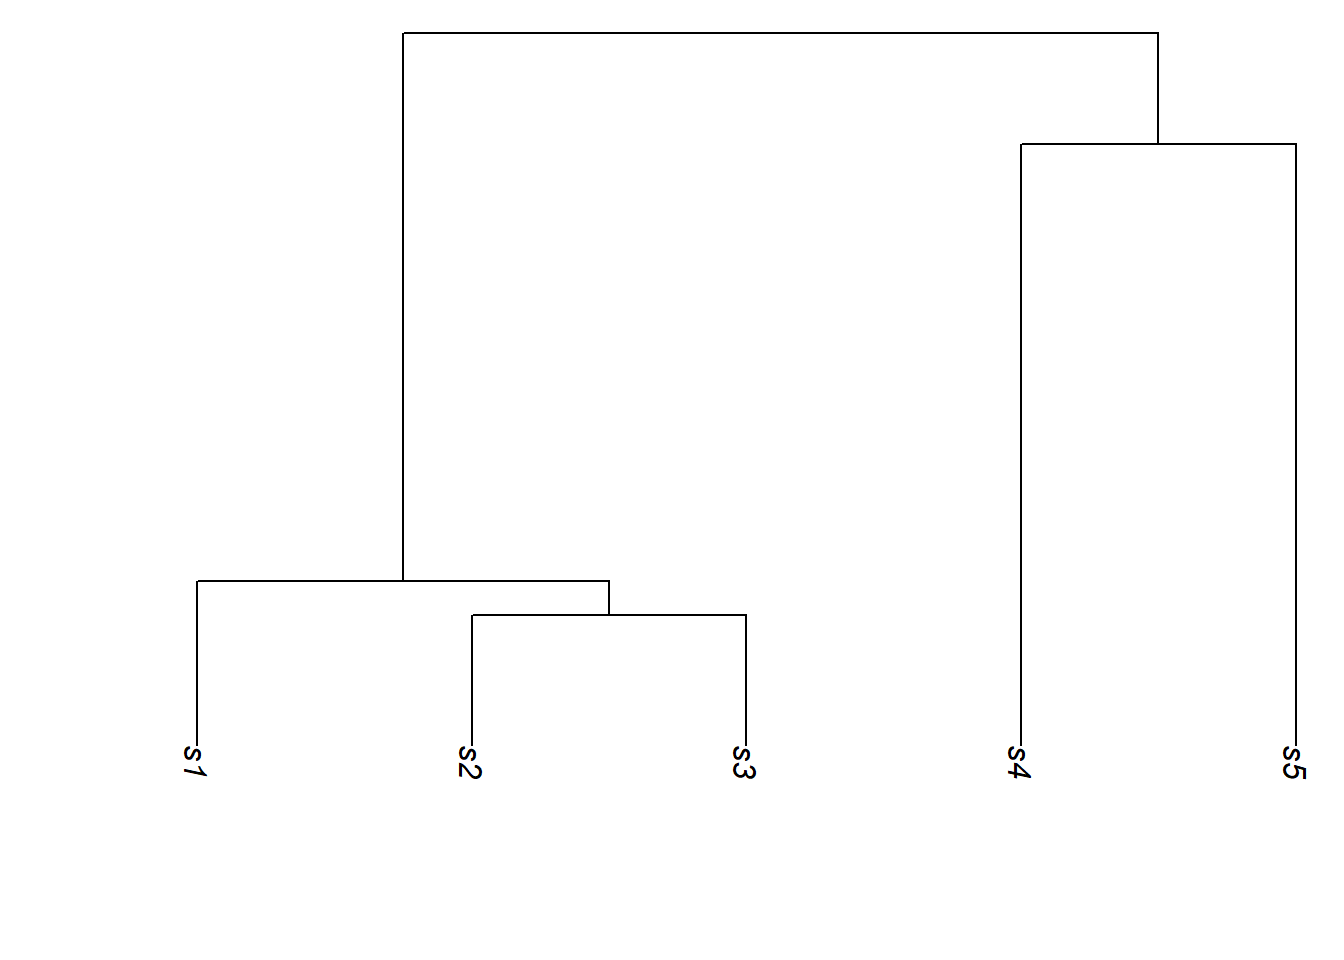
\includegraphics{_main_files/figure-latex/unnamed-chunk-1-1} 

}

\caption{Gene Genealogy with 5 samples: Bifurcated Tree with root not shown}\label{fig:unnamed-chunk-1}
\end{figure}

5 Sequences \{\emph{s1, s2, s3, s4, s5}\} are drawn at the current time \(t=0\) and going back in time, pairs of lineages merge together. The internal nodes denote the common ancestors of the pair of lineages merging into it. Starting with \(n\) samples, (\(n=5\) in the above figure), there are \(n-1\) internal nodes and a total of \(2n-2\) branches with \(n\) external branches \emph{connecting the tips to the internal nodes} and \(n-2\) internal branches connecting the internal nodes.

\hypertarget{an-unnumbered-section}{%
\subsection*{An unnumbered section}\label{an-unnumbered-section}}
\addcontentsline{toc}{subsection}{An unnumbered section}

Chapters and sections are numbered by default. To un-number a heading, add a \texttt{\{.unnumbered\}} or the shorter \texttt{\{-\}} at the end of the heading, like in this section.

\hypertarget{the-coalescent}{%
\chapter{The Coalescent}\label{the-coalescent}}

After introducing and defining genealogies in the previous chapter, John Wakeley talks about the statistical properties of genealogies under the coalescent framework. To demonstrate the coalescent framework, he uses the classical population genetics models: a. Wright Fisher Model b. Moran Model and shows these models converging to the Coalescent in the limit.

Throughout this chapter, there is no reference to variation in sequences with the following two reasons: 1. A sample without any variation still supports a genealogy, because of the way DNA replication takes place. 2. All variation is assumed to be selectively neutral (any selection is dealt later in the book) and so there is no population advantage with respect to any particular variation.

\hypertarget{basic-population-genetic-models}{%
\section{Basic Population Genetic Models}\label{basic-population-genetic-models}}

\hypertarget{wright-fisher-model}{%
\subsection*{Wright Fisher Model}\label{wright-fisher-model}}
\addcontentsline{toc}{subsection}{Wright Fisher Model}

\begin{itemize}
\tightlist
\item
  Perfectly non-overlapping generations
\item
  Population size is constant and finite at all times
\item
  Each generation all current individuals die and are replaced by their offsprings. This is a random process with the possibility that a current individual has no offsprings in the next generation. For any individual in the next generation, any individual in the current generation has an equal chance of being a parent.
\end{itemize}

Let's consider a simple example of a population with two alleles \textbf{A} and \textbf{B} following the WF model. Let the population size be \(N\) and \(K_t\) be the no. of \textbf{A} alleles in generation \(t\) with \(K_0 = i\). Then the probability that the \(K_1 = j\) is given by: \[\mathbb{P}_{ij} = {N \choose j}\left(\frac{i}{N}\right)^j\left(1-\frac{i}{N}\right)^{N-j}\] We also have that the expected number and variance of \textbf{A} alleles in generation \(1\) as \[\begin{align*} & \mathbb{E}(K_1) = N\left(\frac{i}{N}\right) = i \\ & \mathbb{V}ar(K_1) = N \left(\frac{i}{N}\right) \left(1 - \frac{i}{N}\right) = i\left(1-\frac{i}{N}\right)  \end{align*}\] The expected number of \textbf{A} alleles remains unchanged over time.

\hypertarget{moran-model}{%
\subsection*{Moran Model}\label{moran-model}}
\addcontentsline{toc}{subsection}{Moran Model}

There are two steps to cross-reference any heading:

\begin{enumerate}
\def\labelenumi{\arabic{enumi}.}
\tightlist
\item
  Label the heading: \texttt{\#\ Hello\ world\ \{\#nice-label\}}.

  \begin{itemize}
  \tightlist
  \item
    Leave the label off if you like the automated heading generated based on your heading title: for example, \texttt{\#\ Hello\ world} = \texttt{\#\ Hello\ world\ \{\#hello-world\}}.
  \item
    To label an un-numbered heading, use: \texttt{\#\ Hello\ world\ \{-\#nice-label\}} or \texttt{\{\#\ Hello\ world\ .unnumbered\}}.
  \end{itemize}
\item
  Next, reference the labeled heading anywhere in the text using \texttt{\textbackslash{}@ref(nice-label)}; for example, please see Chapter.

  \begin{itemize}
  \tightlist
  \item
    If you prefer text as the link instead of a numbered reference use: {[}any text you want can go here{]}.
  \end{itemize}
\end{enumerate}

\hypertarget{captioned-figures-and-tables}{%
\section{Captioned figures and tables}\label{captioned-figures-and-tables}}

Figures and tables \emph{with captions} can also be cross-referenced from elsewhere in your book using \texttt{\textbackslash{}@ref(fig:chunk-label)} and \texttt{\textbackslash{}@ref(tab:chunk-label)}, respectively.

See Figure \ref{fig:nice-fig}.

\begin{Shaded}
\begin{Highlighting}[]
\FunctionTok{par}\NormalTok{(}\AttributeTok{mar =} \FunctionTok{c}\NormalTok{(}\DecValTok{4}\NormalTok{, }\DecValTok{4}\NormalTok{, .}\DecValTok{1}\NormalTok{, .}\DecValTok{1}\NormalTok{))}
\FunctionTok{plot}\NormalTok{(pressure, }\AttributeTok{type =} \StringTok{\textquotesingle{}b\textquotesingle{}}\NormalTok{, }\AttributeTok{pch =} \DecValTok{19}\NormalTok{)}
\end{Highlighting}
\end{Shaded}

\begin{figure}

{\centering 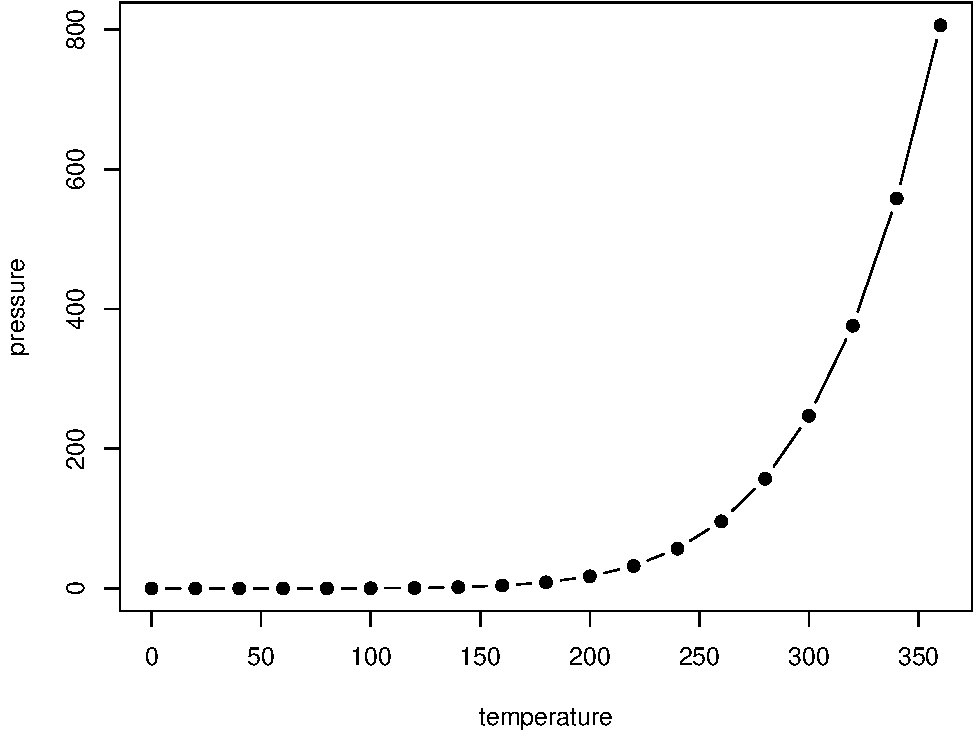
\includegraphics[width=0.8\linewidth]{_main_files/figure-latex/nice-fig-1} 

}

\caption{Here is a nice figure!}\label{fig:nice-fig}
\end{figure}

Don't miss Table \ref{tab:nice-tab}.

\begin{Shaded}
\begin{Highlighting}[]
\NormalTok{knitr}\SpecialCharTok{::}\FunctionTok{kable}\NormalTok{(}
  \FunctionTok{head}\NormalTok{(pressure, }\DecValTok{10}\NormalTok{), }\AttributeTok{caption =} \StringTok{\textquotesingle{}Here is a nice table!\textquotesingle{}}\NormalTok{,}
  \AttributeTok{booktabs =} \ConstantTok{TRUE}
\NormalTok{)}
\end{Highlighting}
\end{Shaded}

\begin{table}

\caption{\label{tab:nice-tab}Here is a nice table!}
\centering
\begin{tabular}[t]{rr}
\toprule
temperature & pressure\\
\midrule
0 & 0.0002\\
20 & 0.0012\\
40 & 0.0060\\
60 & 0.0300\\
80 & 0.0900\\
\addlinespace
100 & 0.2700\\
120 & 0.7500\\
140 & 1.8500\\
160 & 4.2000\\
180 & 8.8000\\
\bottomrule
\end{tabular}
\end{table}

\hypertarget{neutral-genetic-variation}{%
\chapter{Neutral Genetic Variation}\label{neutral-genetic-variation}}

You can add parts to organize one or more book chapters together. Parts can be inserted at the top of an .Rmd file, before the first-level chapter heading in that same file.

Add a numbered part: \texttt{\#\ (PART)\ Act\ one\ \{-\}} (followed by \texttt{\#\ A\ chapter})

Add an unnumbered part: \texttt{\#\ (PART\textbackslash{}*)\ Act\ one\ \{-\}} (followed by \texttt{\#\ A\ chapter})

Add an appendix as a special kind of un-numbered part: \texttt{\#\ (APPENDIX)\ Other\ stuff\ \{-\}} (followed by \texttt{\#\ A\ chapter}). Chapters in an appendix are prepended with letters instead of numbers.

\hypertarget{the-structured-coalescent}{%
\chapter{The Structured Coalescent}\label{the-structured-coalescent}}

\hypertarget{footnotes}{%
\section{Footnotes}\label{footnotes}}

Footnotes are put inside the square brackets after a caret \texttt{\^{}{[}{]}}. Like this one \footnote{This is a footnote.}.

\hypertarget{citations}{%
\section{Citations}\label{citations}}

Reference items in your bibliography file(s) using \texttt{@key}.

For example, we are using the \textbf{bookdown} package \citep{R-bookdown} (check out the last code chunk in index.Rmd to see how this citation key was added) in this sample book, which was built on top of R Markdown and \textbf{knitr} \citep{xie2015} (this citation was added manually in an external file book.bib).
Note that the \texttt{.bib} files need to be listed in the index.Rmd with the YAML \texttt{bibliography} key.

The RStudio Visual Markdown Editor can also make it easier to insert citations: \url{https://rstudio.github.io/visual-markdown-editing/\#/citations}

\hypertarget{separation-of-time-scales}{%
\chapter{Separation of Time Scales}\label{separation-of-time-scales}}

\hypertarget{equations}{%
\section{Equations}\label{equations}}

Here is an equation.

\begin{equation} 
  f\left(k\right) = \binom{n}{k} p^k\left(1-p\right)^{n-k}
  \label{eq:binom}
\end{equation}

You may refer to using \texttt{\textbackslash{}@ref(eq:binom)}, like see Equation \eqref{eq:binom}.

\hypertarget{theorems-and-proofs}{%
\section{Theorems and proofs}\label{theorems-and-proofs}}

Labeled theorems can be referenced in text using \texttt{\textbackslash{}@ref(thm:tri)}, for example, check out this smart theorem \ref{thm:tri}.

\begin{theorem}
\protect\hypertarget{thm:tri}{}\label{thm:tri}For a right triangle, if \(c\) denotes the \emph{length} of the hypotenuse
and \(a\) and \(b\) denote the lengths of the \textbf{other} two sides, we have
\[a^2 + b^2 = c^2\]
\end{theorem}

Read more here \url{https://bookdown.org/yihui/bookdown/markdown-extensions-by-bookdown.html}.

\hypertarget{callout-blocks}{%
\section{Callout blocks}\label{callout-blocks}}

The R Markdown Cookbook provides more help on how to use custom blocks to design your own callouts: \url{https://bookdown.org/yihui/rmarkdown-cookbook/custom-blocks.html}

\hypertarget{ancestral-graphs}{%
\chapter{Ancestral Graphs}\label{ancestral-graphs}}

\hypertarget{publishing}{%
\section{Publishing}\label{publishing}}

HTML books can be published online, see: \url{https://bookdown.org/yihui/bookdown/publishing.html}

\hypertarget{pages}{%
\section{404 pages}\label{pages}}

By default, users will be directed to a 404 page if they try to access a webpage that cannot be found. If you'd like to customize your 404 page instead of using the default, you may add either a \texttt{\_404.Rmd} or \texttt{\_404.md} file to your project root and use code and/or Markdown syntax.

\hypertarget{metadata-for-sharing}{%
\section{Metadata for sharing}\label{metadata-for-sharing}}

Bookdown HTML books will provide HTML metadata for social sharing on platforms like Twitter, Facebook, and LinkedIn, using information you provide in the \texttt{index.Rmd} YAML. To setup, set the \texttt{url} for your book and the path to your \texttt{cover-image} file. Your book's \texttt{title} and \texttt{description} are also used.

This \texttt{gitbook} uses the same social sharing data across all chapters in your book- all links shared will look the same.

Specify your book's source repository on GitHub using the \texttt{edit} key under the configuration options in the \texttt{\_output.yml} file, which allows users to suggest an edit by linking to a chapter's source file.

Read more about the features of this output format here:

\url{https://pkgs.rstudio.com/bookdown/reference/gitbook.html}

Or use:

\begin{Shaded}
\begin{Highlighting}[]
\NormalTok{?bookdown}\SpecialCharTok{::}\NormalTok{gitbook}
\end{Highlighting}
\end{Shaded}

\hypertarget{simulations-and-inference}{%
\chapter{Simulations and Inference}\label{simulations-and-inference}}

Notes to be added

  \bibliography{book.bib,packages.bib}

\end{document}
